% Chapter Template

\chapter{Conclusion} % Main chapter title

\label{Chapter7} % Change X to a consecutive number; for referencing this chapter elsewhere, use \ref{ChapterX}

\lhead{Chapter 7. \emph{Conclusions}} % Change X to a consecutive number; this is for the header on each page - perhaps a shortened title

%----------------------------------------------------------------------------------------
%	SECTION 1
%----------------------------------------------------------------------------------------

Low mass SUSY has been deeply constrained during run 1, however, 
the central motivation -- to stabilise the Higgs mass naturally -- remains. 
The LHC upgrade will provide significantly increased energies and luminosities. The predicted 
probability for production of SUSY sparticles will be significantly 
increased  \cite{ProjectedCx}. In order to have the sensitivity to discover this new physics 
an effective search strategy is crucial. Improvements have been 
made to the object definitions allowing cleaner signal and control
samples. An electron control sample has also been added to allow
greater predictive power for electroweak backgrounds. Finally, the way in which
the data is categorised has been significantly changed in order to take much better
advantage of the difference in the \mht shape between signal and
background while remaining data driven. It will be crucial in early data to study the QCD contamination as well as evaluate the size and effect of all systematics. If low mass SUSY is physical then 
the LHC upgrade and \alphat will provide an excellent opportunity for discovery. 

%\begin{figure}
%\centering
 %   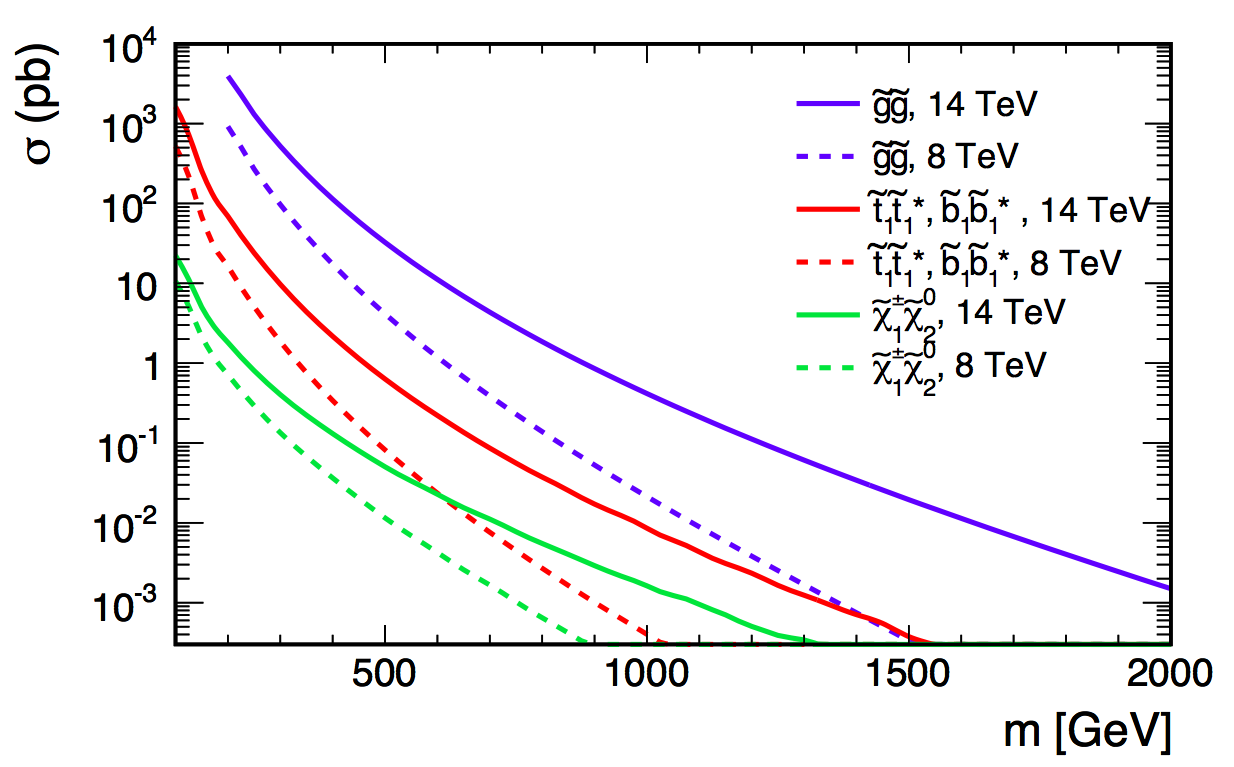
\includegraphics[width=0.7\textwidth]{Figures/snowmass.png}
 % \caption{SUSY production cross sections at 14 TeV compared with 8TeV}
 % \label{snow}
%\end{figure}


